%!TEX root = ../main.tex

% Notes 

\chapter{Related Works}

\section{Hardware Definition Languages (HDL)}

Hardware description languages like Verilog and VHDL are designed for arbitrary circuit description.
Initially, these languages are developed as hardware simulation languages, and were only later adopted as a basis for hardware design.
While HDL language syntaxes' resemble software languages but they concepts are inherently different from software languages.
Software programs are inherently design to describe an algorithm for processors.
They have sequential semantics and correctness of the program is defined as executing instructions in the order it is written. Data movement is implicit between instructions and there is a explicit defined memory model.
In contrast, HLD languages are designed to specify circuit designs.
Hardware inherently is concurrent, therefor, each statement in HDL language is concurrent with other statements.
All the dependencies need to be explicit either in the form of wire or register.
There is no pre-defined memory model. Memory model needs to be explicitly defined and handled in the design.
Because the semantics of these languages are based around simulation, synthesizable designs must be inferred from a subset of the language, complicating tool development and designer education.
They can result in ambiguities that make automated synthesis and verification impossible, due to the unclear semantics involved.
For any design in order to achieve maximum generality, they require users to explicitly manage timing, control signals, and local memories.

A big limitation of HDL languages is that these languages lack the powerful abstraction facilities that
are common in modern software languages, which leads to low designer productivity by making it difficult to reuse components~\cite{shacham_rethinking_2010}.
Constructing efficient hardware designs requires extensive design-space exploration of alternative system microarchitectures but traditional HLDs have limited module generation facilities and are ill-suited to producing and composing the highly parameterized module generators required to support through design-space exploration.
Recent extensions such as SystemVerilog improve the type system and parameterized generate facilities but still lack many powerful programming language features.
But why reusing components is important?
The key benefit of reusing hardware components is that every time a chip is built, we inherently evaluate different design decisions, either implicitly using microarchitectural and domain knowledge, or explicitly through custom evaluation tools.
Rather than building a custom chip, designers create a template, or a chip generator, that can generate the specialized chip. Tensilica applied the same idea to create customized processors~\cite{tensillica}~\cite{tensillica}.

\subsection{BlueSpec}

Another alternative proposal to improve productivity of HLD languages was beginning from a domain-specific application programming language and then generate hardware blocks. 
Bluespec~\cite{bluespec} is an example of such languages.
Bluespec Compiler (BSC) is a tool that uses BluespecSystem  Verilog  (BSV)  as  the  design  language.
BSV is a high-level functional HDL based on Verilog and inspired by Haskell, where  modules are implemented as a set of rules using  Verilog  syntax.
In this language, the concurrent behavior of a system is expressed as a collection of rewrite rules.
The rules are called guarded atomic actions and express behavior in the form of concurrently cooperating finite state machines (FSMs).
Rules are predicated with a condition. They give the impression of freezing the rest of the system when a given rule's action is carried out after the rule's predicate is true.
There is an implicit parallelism in this specification, because it is possible for multiple rules to be activated and executed in parallel.
The compiler automatically schedules the rules such that they are either conflict-free or combined sequentially to preserve the promised atomicity semantic.

While these can provide great designer productivity when the task in hand matches the pattern encoded in the application programming model, they are a poor match for tasks outside their domain.
For example, the design of a programmable microprocessor is not well described in a stream
programming model, and guarded atomic actions are not a natural way to express a high-level DSP algorithm.
Furthermore, in general it is difficult to derive an efficient microarchitecture from a higher-level computation model, especially if the goal is a programmable engine to run many applications, where the human designer would prefer to write a generator to explore this design space in detail.


\section{Hardware Constructor Languages (HCL)}


\subsection{Genesis2}
Genesis2~\cite{genesis2} was one of the first attempts to work around these limitations. Genesis2 uses Perl language as a macro processing language to provide more flexible parameterization and elaboration of underlying hardware blocks in SystemVerilog. Listing~\ref{listing:genesis2} shows an example of \textit{Genesis2's code}.
In this example, perl is using ceil library from POSIX library to set the values for $\$num\_add\_bits$.

\begin{listing}[ht]
    \begin{minted}{Verilog}
        //; # More Perl Libraries
        //; use POSIX (ceil);
        //; my $reg_list = $self->define_param(REG_LIST => 
        //; [	
        //;     {name => 'regA', width => 5, default => 17, IEO => 'ie'},
        //;     {name => 'regB', width => 15, IEO => 'ieo'},
        //;     {name => 'regC', width => 32, IEO => 'ieo'},
        //; ]);
        //; my $num_regs = scalar(@{$reg_list});
        //; my $num_addr_bits = ceil(log($num_regs)/log(2));

        // Verilog code for the module
        module 'mname()' (
            input                               Clk,
            input                               Reset,
            input ['$num_addr_bits-1':0]        Addr,
            ...
            );

        endmodule // 'mname()'
    \end{minted}
    \caption[Caption for LOF]%
    {Genesis2 code example, combining SystemVerilog and Perl~\cite{genesis2}}
    \label{listing:genesis2}
\end{listing}


These approaches allow familiar and powerful languages like Verilog to be macro languages for hardware netlists, but effectively require leaf components of the design to be described in the underlying HDL.
This combined approach is cumbersome, combining the poor abstraction facilities of the underlying HDL with a completely different high-level programming model that does not understand hardware types and semantics.

\subsection{Chisel and FIRRTL}

Chisel~\cite{chisel} is another successful, modern, generalize HCL which is a domain specific language (DSL) for describing hardware circuits embedded in Scala.
Chisel provides modern programming language features such as meta-programming and object oriented concept coupled with library availability for accurately specifying low-level hardware blocks, but which can be readily extended to capture many useful high-level hardware design patterns.

There is a question that always exist about HCL languages versus HDLs. The question is that \emph{What benefits does Chisel offer over classic Hardware Description Langues?\footnote{\url{https://github.com/freechipsproject/chisel3}}}
There are two main angles: 1)Chisel improved productivity through new language features and availability of reusable libraries. 2)Improved specialization due to the hardware-compiler structure. We elaborate more on these two angles in the continue.
Chisel by itself do not provide any new hardware abstractions. However, host language features, Scala, allow designs to be more parameterizable and modular~\cite{izraelevitz_2017_firrtl_reusability}.
For instance,  someone can write a recursive Scala function to construct an adder-reduction tree, parameterized on bit-width.
Unlike the explicitly unrolled version necessary in Verilog, the same generator could be re-used anywhere an adder tree is desired.
Figure~\ref{fig:filter} shows the specified example and the abstract Chisel code.

\begin{figure}[h]
    \centering
    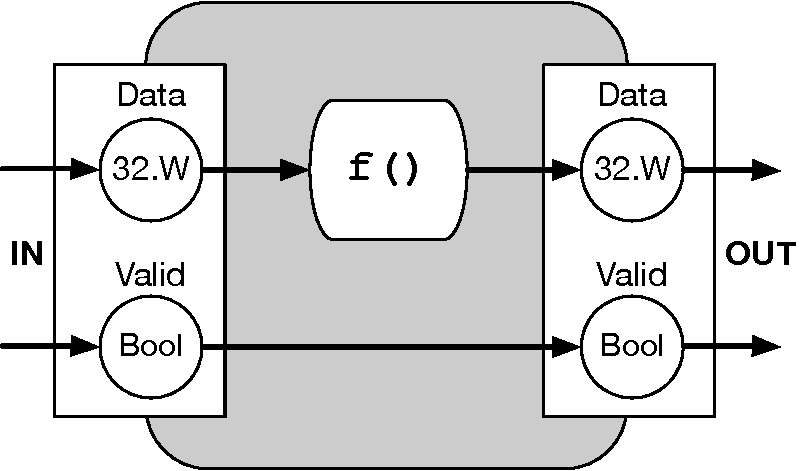
\includegraphics[width=0.45\textwidth]{figures/Introduction/Filter.pdf}
    \caption{Missing Semantics}
    \label{fig:filter}
\end{figure}


\begin{listing}[ht]
    \begin{minted}{Scala}

    abstract class Filter[T <: Data](dtype: T) extends Module {
    val io  = new Bundle {
    val in  = Input(Valid(dtype))
    val out = Output(Valid(dtype))
    } }

    class FunctionFilter[T <: Data](dtype: T, f: T => T) extends Filter(dtype) {
    io.out.valid := io.in.valid
    io.out.bits := f(io.in)
    }

    \end{minted}
    \caption{Chisel abstract function filter}
    \label{listing:genesis2}
\end{listing}




In another example, designer can write a filter module which takes, as a parameter, a higher-order-function that creates the condition checking hardware.
The user of this module then only needs to write the filtering condition, re-using the base filter structure.
There are mature Chisel projects like \emph{Rocket-Chip~\cite{rocket-chip}} and \emph{Diplomacy~\cite{diplomacy}} as other examples for showing Chisel's power as hardware construction language.
The second bold advantage of Chisel compare to HDLs is a Hardware Compiler Framework that looks very much like LLVM~\cite{llvm} applied to hardware generation.
The Chisel-to-Verilog process forms part of a multi-stage compiler.
The "Chisel stage/front-end" compiles Chisel to a circuit intermediate representation called FIRRTL (Flexible Intermediate Representation for RTL)~\cite{firrtl}.
"FIRRTL stage/mid-end" then optimizes FIRRTL and applies user-custom transformations. Finally the "Verilog stage/back-end" emits Verilog based on the optimized FIRRTL.
In this process FIRRTL represents the standardized elaborated circuit that the Chisel HDL produces.
FIRRTL represents the circuit immediately after Chisel's elaboration but before any circuit simplification.
It is designed to resemble the Chisel after all meta-programming has executed. Thus, a user program that makes little use of meta-programming facilities should look almost identical to the generated FIRRT.

In fact, FIRTTL as the hos language, Chisel, to be used for mostly its met-programming facilities, the Chisel front-end can be very light-weight, and additional HDLs written in other languages can target FIRRTL and reuse the majority of the compiler toolchain.


While these improvements allow for more powerful meta-programming compared to Verilog \code{generate} statements, users still write programs at a timed circuit level. This is still one of the most important limitation of HCLs to improve the overall system design productivity.

\section{Spatial}
% * Spatial~\cite{david_PLDI_2018_spatial, prabhakar_asplos_2016_parallelpattern}
% * A practice to improve chisel flexibility
% * Higher level of abstraction to chisel
% * Untimed modules
% * Reduction to parallel patterns
Recently, Spatial~\cite{david_PLDI_2018_spatial} is been proposed as a language and compiler for applications specific accelerators.
Spatial focuses on specific type of high-level abstractions required to create a new high level HDL language in which syntax contains memory, control and accelerator-host interface as an individual entity.
Spatial claims these particular constructs within the language are better fit for accelerators specially targeting applications with data locality and data parallelism.
Spatial tries to reduce productivity gap by increasing level of abstraction at the structure domain. Spatial expresses accelerators with untimed module, nested loops and customized memory hierarchy.
The most advantage of Spatial is limiting the design to these set of constructs and it allows compiler to more easily optimize designs.
Spatial in fact, is a new DSL language on top of Chisel which tries to strike balance between high-level constructs in the language for improving programmer productivity versus low-level syntax for tuning performance. 
For instance, to enable the compiler to be able to reason about the loop structures, Spatial limits the types of control structures to four types: FSMs, Foreach, Reduce and MapReduce. 
Therefore, as long as the hardware accelerator designer can express his design in such patterns, compiler can reason about the available parallelism and automatically pipeline the design.
However, in many cases such control structures are note enough to express arbitrary designs.

While Spatial has improved the accelerator design productivity compare to classic HDL designs.
But still to design a specific accelerator design needs to re-implement the accelerator's design in Spatial language. Moreover, Spatial is not designed to be target by high level synthesis tools.
Therefore, it can not support synthesizing arbitrary designs from behavioral description.
The main goal of Spatial is limiting DSE by defining higher level abstractions on top of Chisel and enabling compiler to only search trough very limited space.

\subsection{High-Level Synthesis}

High-level synthesis (HLS) techniques have been proposed to improve the productivity of hardware designers by automatically generating the hardware from a high-level description of an application.
In pure C-to-gates HLS front-end which captures system behavior with a model of computation in a standard language such as C, C++, SystemC as an input, in the form of untimed nested parallel loops.
In the next step, the compiler tries to statically schedule the input algorithm and applies optimizations such as inner loop pipelining, unrolling, and memory banking and buffering~\cite{chung_micro_2010, lee_1989_new, paulin_1989_force}.
Examples of such HLS tools are LegUp~\cite{canis_2011_legup}, Vivado HLS~\cite{vivadohls}, Intel’s FPGA SDK for OpenCL~\cite{opencl_sdk}, and SDAccel~\cite{sdaccel} allow users to write FPGA designs in C/C++ and OpenCL.
Usually such tools adopt polyhedral tools to automate loop pipelining and banking decisions, but such techniques are limited to only affine accesses withing a single loop nest~\cite{wang_2014_theory}, it does not address non-affine cases or cases where accesses to the same memory occur in multiple loop nests.

To elaborate more on this limitation of standard HLS approaches, consider the code in Listing~\ref{listing:static_schedule}.
In this loop there is a control flow decision (if) which depends on the actual data being read from arrays A[] and B[].
The operation which might take place in a specific iteration (s = s + d) introduces a dependency between iterations and delays the next iteration whenever the condition is true.
A typical HLS tool needs to create a static schedule for the loops, which means it needs to take the conservative decisions for synthesizing the loop. The compiler has either two choices, make the loop serial and state machine base or make the loop iterations pipeline, which for pipelining it usually need input directives from the input algorithm.
Figure~\ref{fig:schedule} shows the both possible schedule for if we use HLS tools that use statically scheduling approach.


\begin{listing}[ht]
    \begin{minted}{C}
        float d, s = 0.0;
        for (int i = 0; i < 100; i++){
            d = A[i] - B[i];
            if (d >= 0)
                s += d:
        }
    \end{minted}
    \caption{Limitations of static scheduling}
    \label{listing:static_schedule}
\end{listing}


\begin{figure}[!h]
    \begin{minipage}[t]{\linewidth}
        \centering
        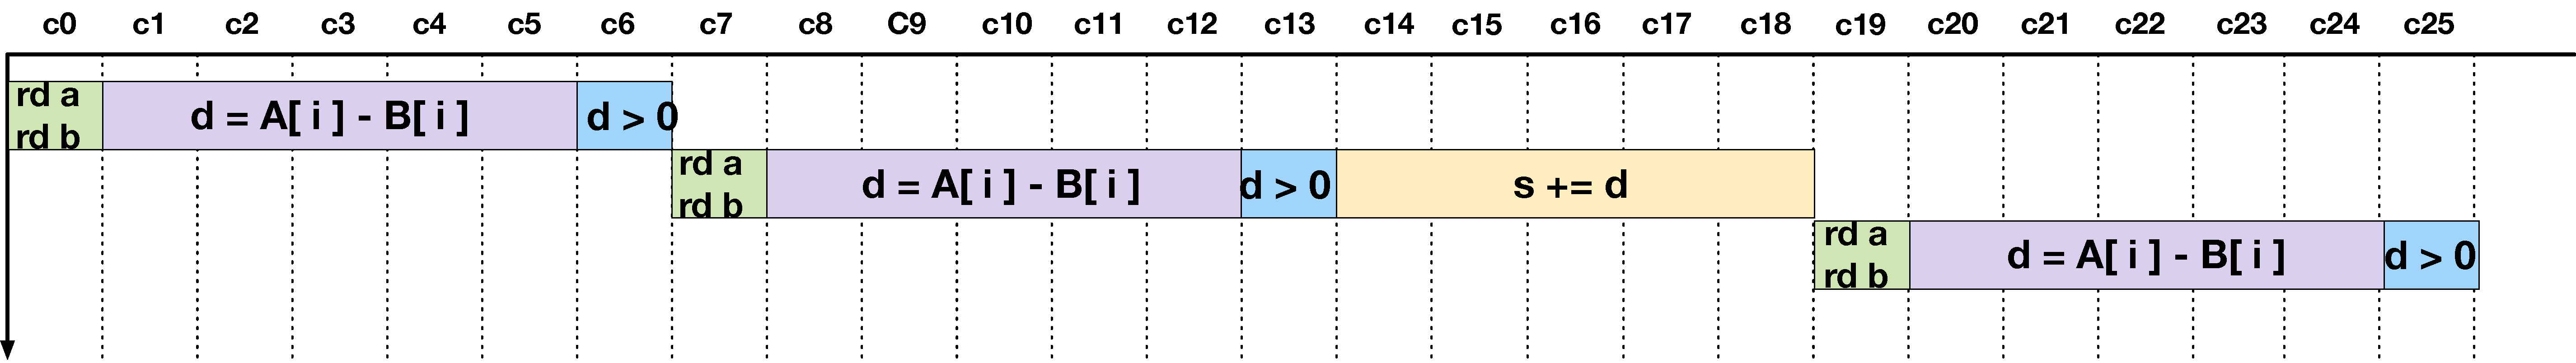
\includegraphics[width=1\textwidth]{figures/Introduction/schedule.pdf}
        \label{fig:no_pipeline}
    \end{minipage}
    \hspace{0.1cm}
    \begin{minipage}[t]{\linewidth} 
        \centering
        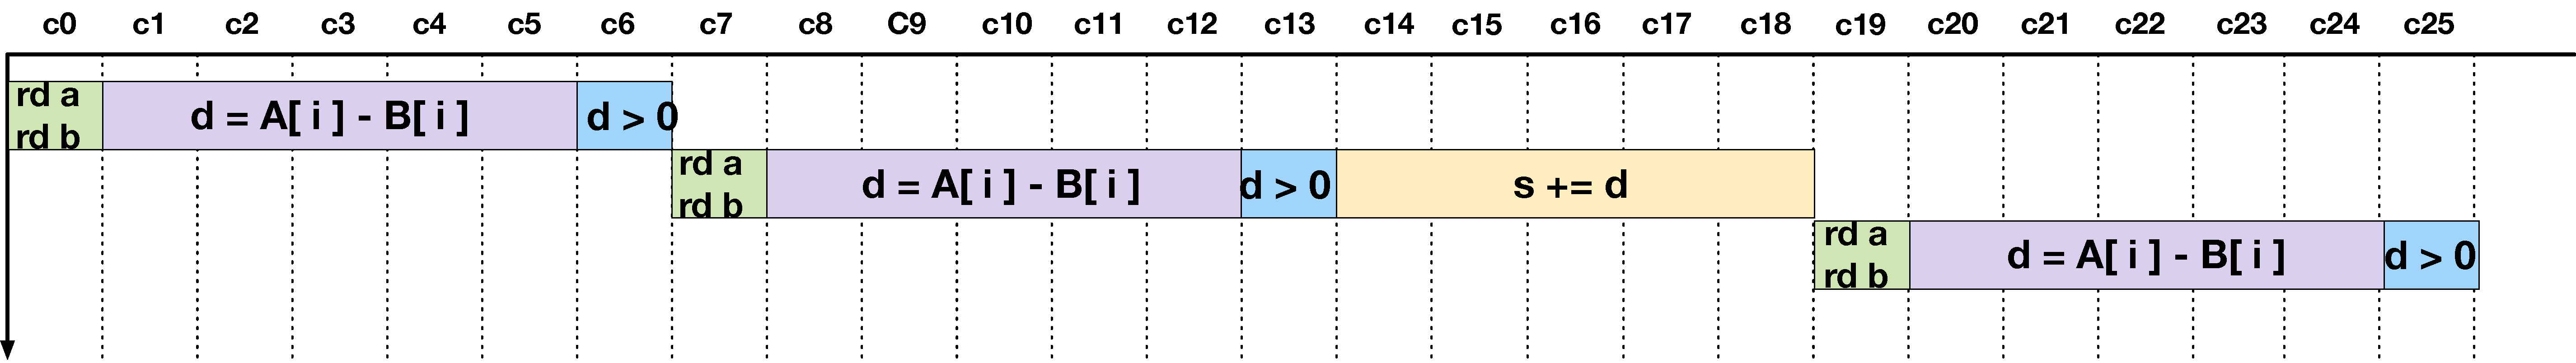
\includegraphics[width=1\textwidth]{figures/Introduction/schedule.pdf}
        \label{fig:pipeline}
    \end{minipage}        
    \label{fig:schedule}
    \caption{Static Schedule: no pipeline}
\end{figure}  





\subsection{Chimps, CASH, AHRL}

Chimps~\cite{chimps}, CASH~\cite{budiu_pegasus_2002,budiu_cash_2002}, AHRL~\cite{ahrl}
% * Generate hardware from ANSI C
% * mapping each C language construct in a dataflow graph to an HDL block.
%

\subsection{ElasticFlow / CGPA}

ElasticFlow~\cite{elasticFlow} / CGPA~\cite{cgpa} / Dynamic schedule dataflow~\cite{josipovic_fpga_2018_dynamically}
% * More recent works like ElasticFlow and CGPA
% * generate coarse-grained pipelines using FIFOs in between stages for communication.
%

\subsection{Gorill}
Gorill~\cite{lavasani_thesis}
% * Gorilla++ generates custom hardware for applications with irregular dataflow 
% * support multi-threading and lock-based synchronization

\subsection{Kiwi}
Kiwi~\cite{kiwi}
% * translates a set of C# parallel constructs to hardware units (monitor, event, lock)
Kiwi translates a set of $C\#$ parallel constructs (e.g., event, monitor,
and lock) to corresponding hardware units.

\subsection{Lime}
Lime~\cite{lime}
% * hardware from functional parallel patterns. (map, reduce, split, join)
% * Java and automatically targets CPUs, GPUs, and FPGAs
%
Lime is a Java-based programming model and runtime from IBM which aims to provide a single unified language to program heterogeneous architectures. Lime natively supports custom bit precisions and includes collection operations, with parallelism in such operations inferred by the compiler. Coarse-grained pipeline and data parallelism are expressed through ``tasks''. Coarse-grained streaming computation graphs can be constructed using built-in constructs like \texttt{\small{connect}}, \texttt{\small{split}}, and \texttt{\small{join}}. The Lime runtime system handles buffering, partitioning, and scheduling of stream graphs. However, coarse-grained pipelines which deviate from the streaming model are not supported, and the programmer has to use a low-level messaging API to handle coarse-grained graphs with feedback loops. Additionally, the compiler does not perform automatic design tuning. Finally, the compiler's ability to instantiate banked and buffered memories is unclear as details on banking multi-dimensional data structures for arbitrary access patterns are not specified.

\subsection{CMOST/ParallelXL}
CMOST~\cite{zhang_DAC_2015_cmost}, ParallelXL~\cite{chen_micro_2018_parallelXL}
% * C-to-FPGA framework that uses task-level modeling



\section{Image Processing DSLs}

\subsection{HIPACC}
HIPACC~\cite{membarth_2016_hipa}
% * source - to - source C like compiler
% * generate CUDA, openCL, Renderscripts target GPU
% * make use of different memory hierarchy based on limit set of access pattern
% * support fix set of reduction function
% * unroll only if kernel size is known
% * heuristic pick best configuration (similar to our DSE)
%

\subsection{Rigel}
Rigel~\cite{hegarty_2016_rigel}
% * Generate verilog
% * Coarse-grain pipeline
% * very similar control semantics to plasticine. Use
% tokens/back pressure to allow each pipeline stage to fire at their perspective rate
% * Multi-rate line buffer template
%

\subsection{Darkroom}
Darkroom~\cite{darkroom}
% * target ASIC, FPGA, fast CPU
% * generate structured verilog
% * line buffer
% * scheduling for inner loop pipeline. Use ILP to improve pipeline delay
%

\subsection{PolyMage}
PolyMage~\cite{mullapudi_asplos_2015_polymage}
% * point=wise, stencil, sampling, operation
% * functional (in a kind of awkward way)
% * python
% * generate openMP/C++
% * generate high-level synthesis tool
% * line buffer


% \subsection{Generators}


\paragraph{Conclusion: } While these improvements allow for more powerful meta-programming compared to Verilog \texttt{\small{generate}} statements, users still write programs at a timed circuit level.

% \subsection{Hardware generator languages}
% \begin{enumerate}
%     \item Chisel, Firrtl
%     \item Rocket core
% \end{enumerate}
